\documentclass{beamer}
\usepackage{amsmath}
\usepackage[utf8]{inputenc}
\usepackage{graphicx}
\usetheme{Warsaw}
\usecolortheme{wolverine}
%\DeclareMathOperator{\taninv}{tan^{-1}}


\title{EE3025 INDEPENDENT PROJECT}
\author{ADITYA PEDAVEGI\\EE18BTECH11034}
\begin{document}
\maketitle
\begin{frame}{Assignment-1 Question 7.1}
The command $output_{signal} = signal.lfilter(b,a,input_{signal})$ in Problem 2.3 is executed with the following difference equation 
\begin{align}
 \sum _{m=0}^{M} a(m)y(n-m) = \sum_{k=0}^{N} b(k)x(n-k)
\end{align}
where input signal is $x(n)$ with initial values all 0.Replace \textbf{signal.filtfilt} with your own routine and verify
\end{frame}

\begin{frame}{Solution}
Computing $X(z)$ from $x(n)$ using inbuilt fft (fast fourier transfrom)command
\begin{align}
X(z) = fft(x(n))
\end{align}
Obtaining $H(z)$ from coefficients b,a as 
\begin{align}
H(z)= \frac{Y(z)}{X(z)} = \frac{\sum _{k=0}^{N}b(k)z^{-k}}{\sum _{m=0}^{M}a(m)z^{-m}}
\end{align}
Obtaining $Y(z)$ as 
\begin{align}
Y(z) = X(z)H(z)
\end{align}
and computing $y(n)$ from $Y(z)$ using inbuit ifft(inverse fast fourier transform) command
\begin{align}
y(n) = ifft(Y(z))
\end{align}
where $y(n)$ is the output signal
\end{frame}
\begin{frame}{Graphical results}
\begin{figure}[!h]
%\centering
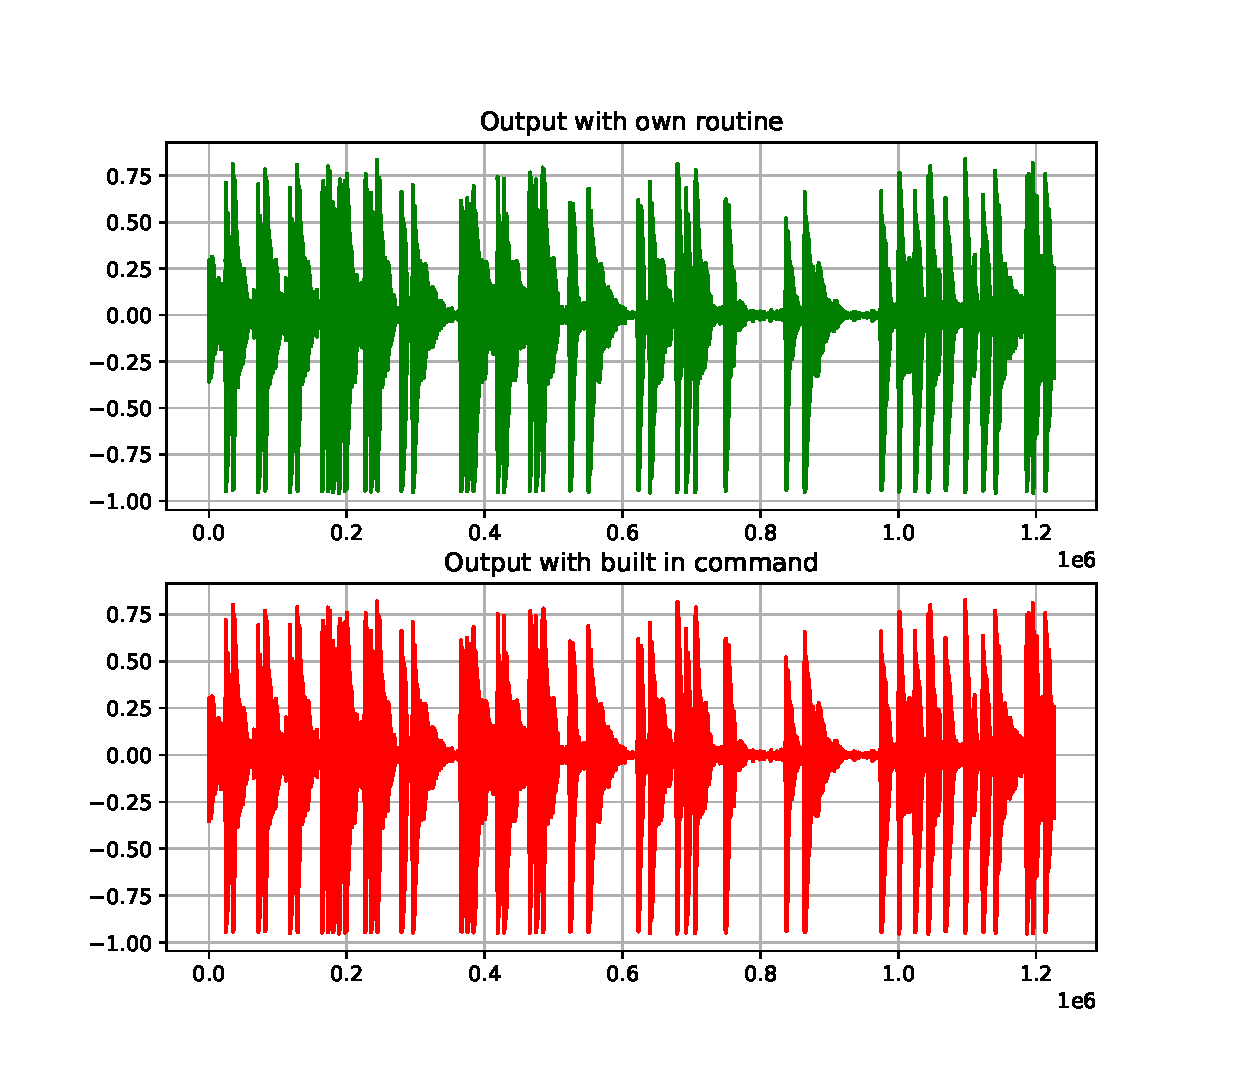
\includegraphics[width=0.75\columnwidth]{./figs/ee18btech11034_1.eps}
\caption{Time domain response of output signal}
\label{fig:Figure1}
\end{figure}
\end{frame}

\begin{frame}
\begin{figure}[!h]
%\centering
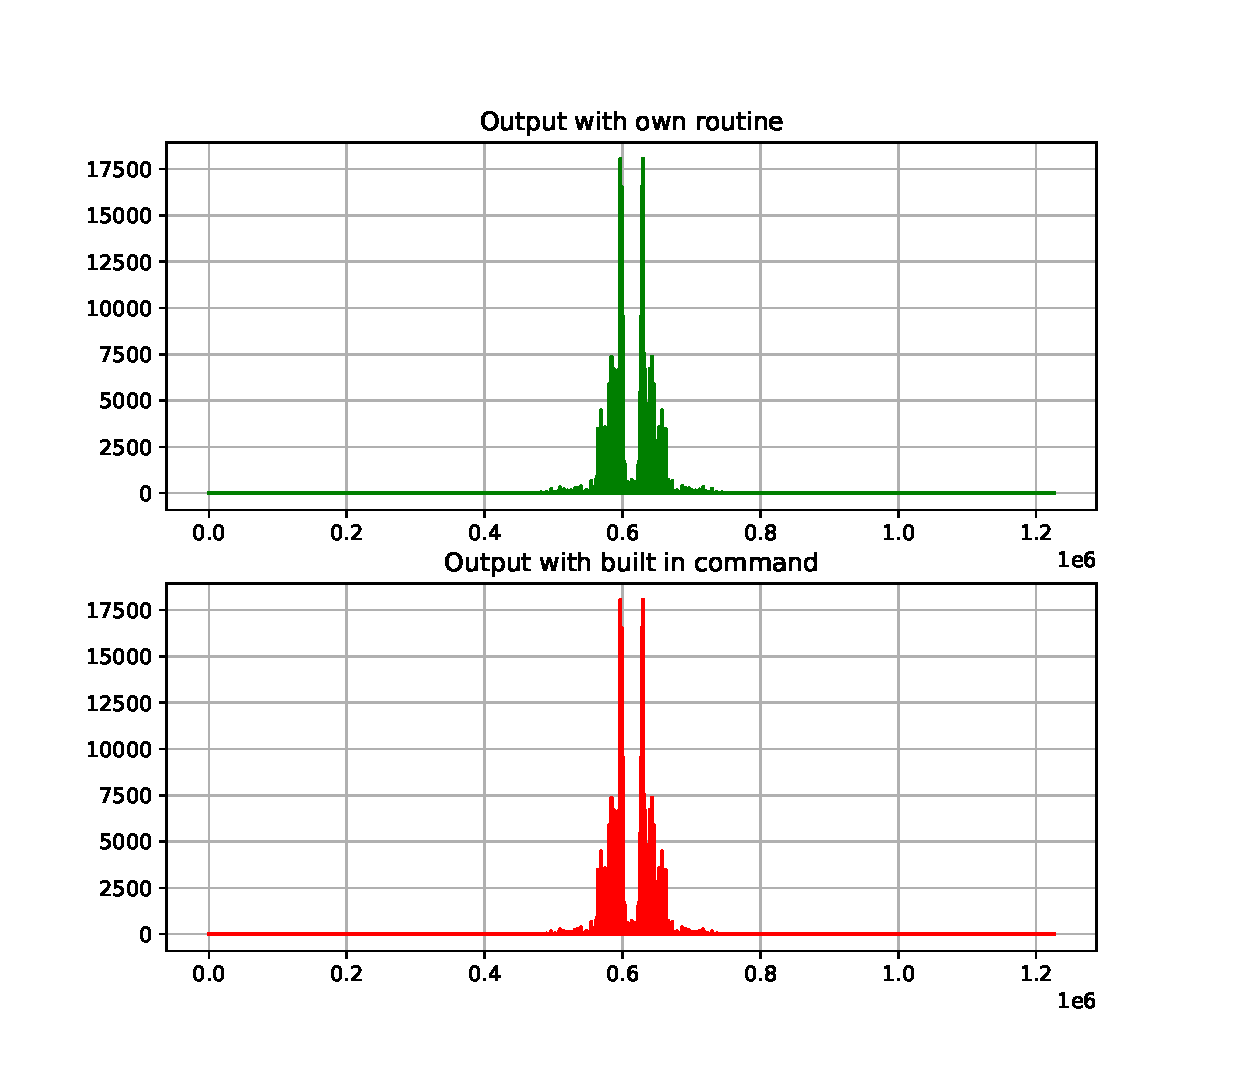
\includegraphics[width=0.75\columnwidth]{./figs/ee18btech11034_2.eps}
\caption{Frequency domain response of output signal}
\label{fig:Figure2}
\end{figure}
\end{frame}
\begin{frame}{FFT Algorithm implementation in C for Assignment-1}
\begin{itemize}
\item Implementing Radix-2 FFT alogorithm making the length of the signal as $N = 2^k$ by appending zeros to the original signal.
\item Spliting the original sequence $x(n)$ into two sequences (even indexing and odd indexing) as $s_1(m) = x(2n)$ and $s_2(m) = x(2n+1)$
\item Now the main DFT expression 
\begin{align}
X(k) = \sum_{n=0}^{N-1} x(n) W_N^{kn} 
\end{align}
where $k=0,1..N-1$ and $W_N = \exp(\frac{-j2\pi}{N})$
\end{itemize}
\end{frame}
\begin{frame}
\begin{itemize}
\item Reduces to the form 
\begin{align}
X(k) = S_1(k) + W_N^kS_2(k)
\end{align}
\begin{align}
X(k+\frac{N}{2}) = S_1(k) - W_N^kS_2(k)
\end{align}
where $k=0,1..\frac{N}{2}-1$, $S_1(k)$ and $S_2(k)$ are $\frac{N}{2}$ point DFT's of the sequences $s_1(m)$ and $s_2(m)$ respectively.
\item Again the $\frac{N}{2}$ point DFT is computed using the same expression above and this is done in a recursive process. 
\end{itemize}
\end{frame}
\begin{frame}{Graphical results}
\begin{figure}[!h]
%\centering
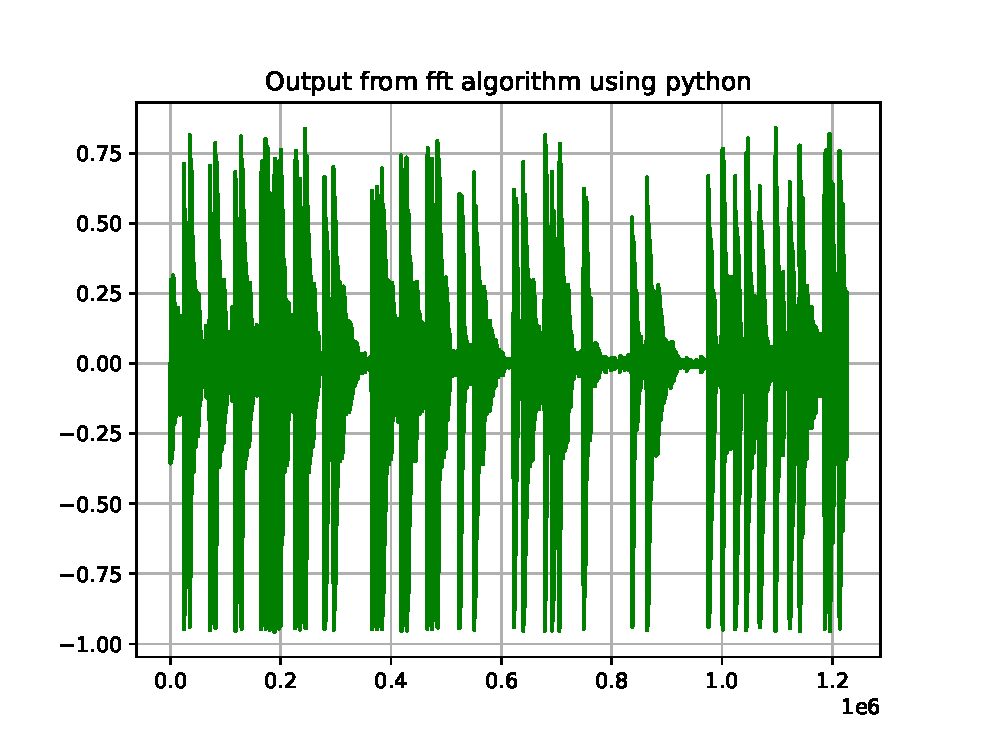
\includegraphics[width=0.30\columnwidth]{./figs/ee18btech11034_3.eps}
\caption{Time domain response in python of output signal}
\label{fig:Figure3}
\end{figure}

\begin{figure}[!h]
%\centering
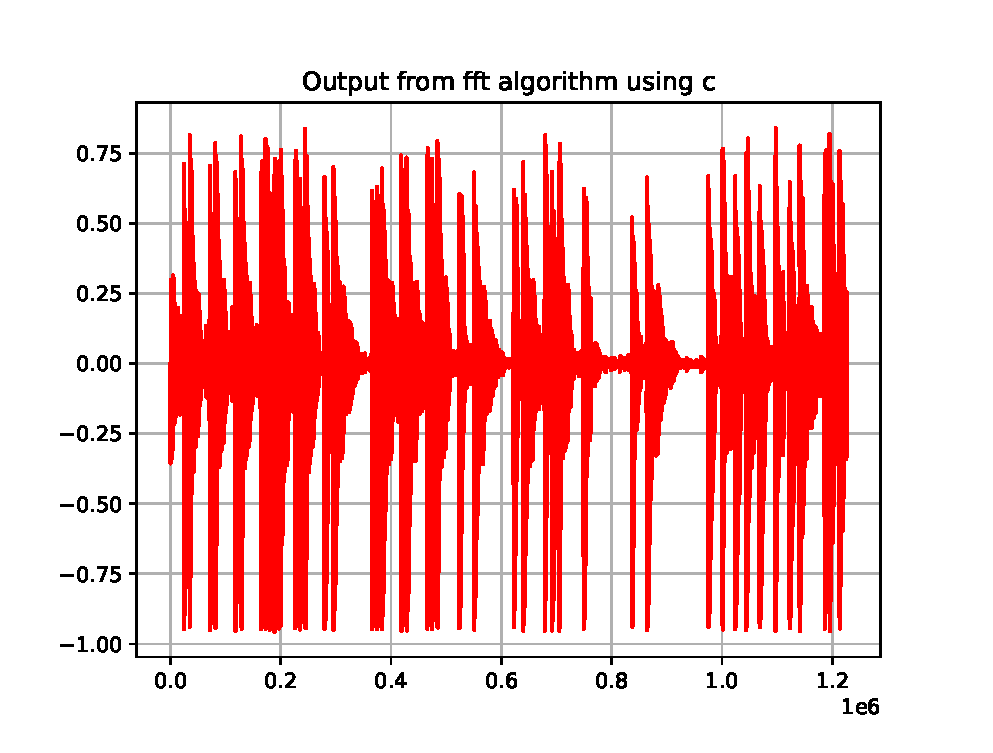
\includegraphics[width=0.30\columnwidth]{./figs/ee18btech11034_4.eps}
\caption{Time domain response in C of output signal}
\label{fig:Figure4}
\end{figure}
\end{frame}
\begin{frame}{Assignment-2 Filter Design}
We are supposed to design FIR and IIR realizations for the filter number 114.Observing magnitude response of the filters.Chebyshev filter is taken in the case of IIR filter
\\
Chebyshev filter have a steeper roll-off than butterworth filter and has stopband monotonic and passband equiripple. 
\end{frame}
\begin{frame}{IIR Filter Design}
After choosing required specifications setting $N=4$ (4th order Chebyshev filter) and $0.3184 < \epsilon < 0.6197$ (parameters of filter), plotting the magnitude response of Lowpass Chebyshev filter for the above values
\\
The transfer function is given as 
\begin{align}
\vert H_{a,LP}(j\Omega_L)\vert^2 = \frac{1}{1 + \epsilon^2c_N^2(\Omega_L)}
\end{align}
where $c_N(x) = \cosh(N \cosh^{-1}x)$ 
\end{frame}
\begin{frame}
\begin{figure}[!h]
%\centering
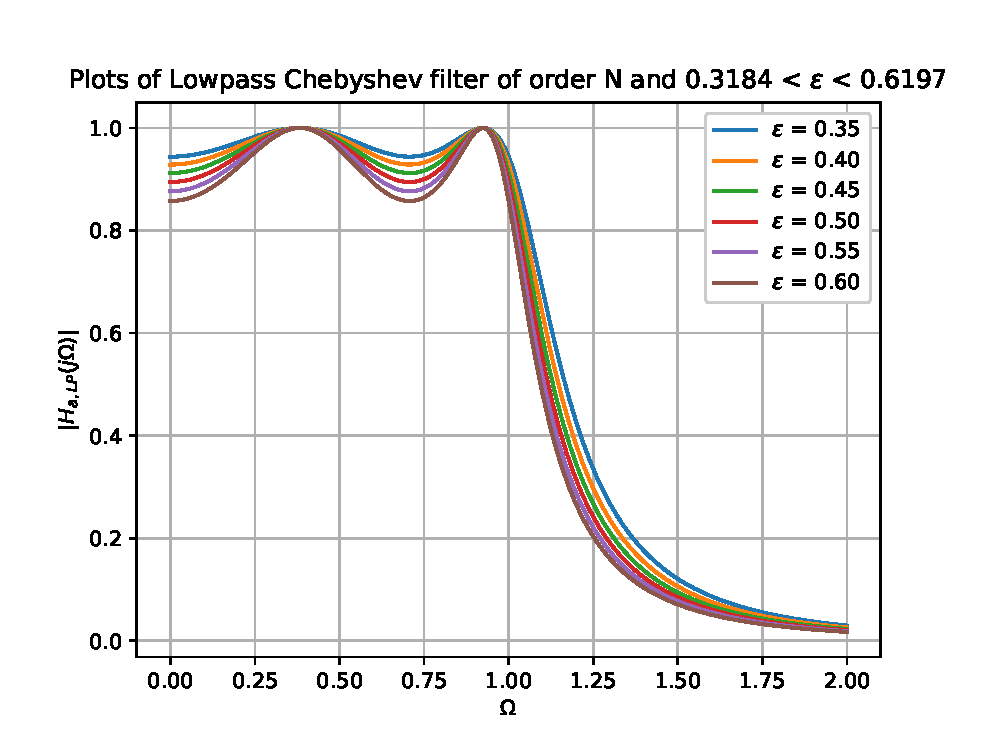
\includegraphics[width=0.75\columnwidth]{./figs_iir/ee18btech11034_parameter_plots.eps}
\caption{Lowpass Chebyshev filter magnitude response for different values of $\epsilon$}
\label{fig:Figure5}
\end{figure}
We choose $\epsilon = 0.4$ for our IIR design
\end{frame}
\begin{frame}
Verifying the design with magnitude response of Lowpass stable Chebyshev filter ($H_{a,LP}(s_L)$) for even order (i.e using Chebyshev polynomial) and obtaining gain as $G_{lp} = 0.3125$ and poles as $p = [1,1.1068,1.6125,0.9140,0.3366]$
\begin{figure}[!h]
%\centering
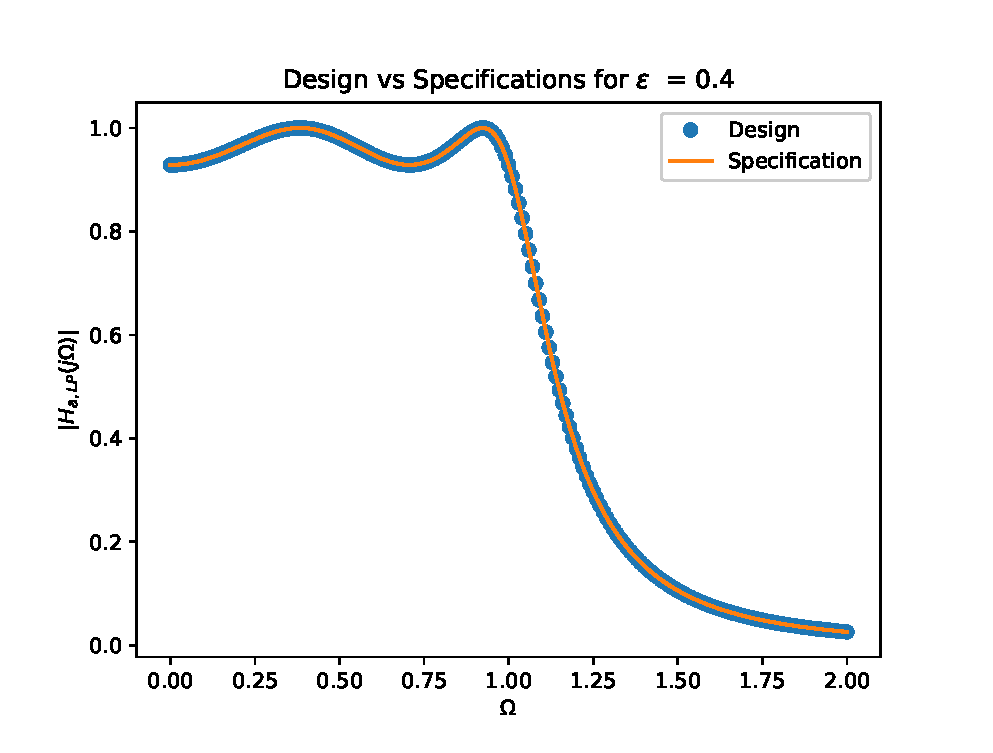
\includegraphics[width=0.75\columnwidth]{./figs_iir/ee18btech11034_specifications.eps}
\caption{Design vs Specifications}
\label{fig:Figure6}
\end{figure}

\end{frame}
\begin{frame}
From the above graph it is verified the design meets the specifications for Lowpass IIR filter.
\\
Obtaining analog band pass Chebyshev filter as
\begin{align}
H_{a,BP}(s) = G_{BP}H_{a,LP}(s_L)
\end{align}
where $G_{BP}$ is gain of analog band pass filter
\\
Obtaining bilinear transformation by substituting $s = \frac{1-z^{-1}}{1+z^{-1}}$ which converts analog filter transfer function to digital filter transfer function and using below equation
\begin{align}
H_{d,BP}(z)  = G_{BP}H_{a,LP}(s)
\end{align}
\end{frame}
\begin{frame}{Plots of Analog Lowpass,Analog Bandpass and Digital Bandpass IIR filters}
\begin{figure}[!h]
%\centering
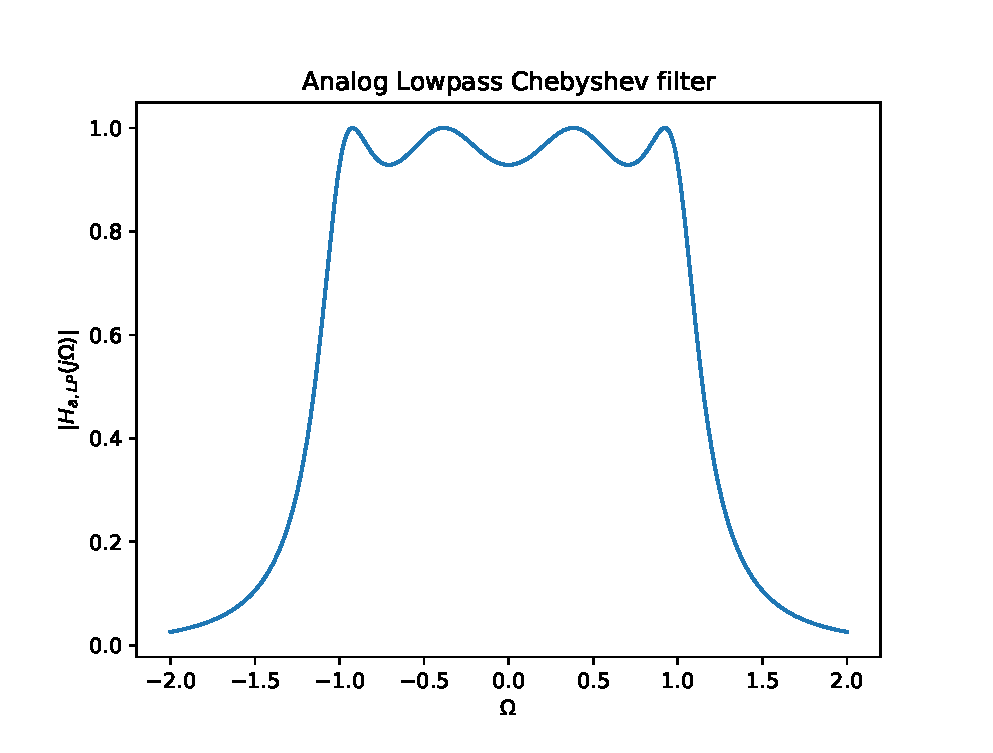
\includegraphics[width=0.30\columnwidth]{./figs_iir/ee18btech11034_Analog_IIR_Lowpass.eps}
\caption{Analog Lowpass IIR filter magnitude response}
\label{fig:Figure7}
\end{figure}

\begin{figure}[!h]
%\centering
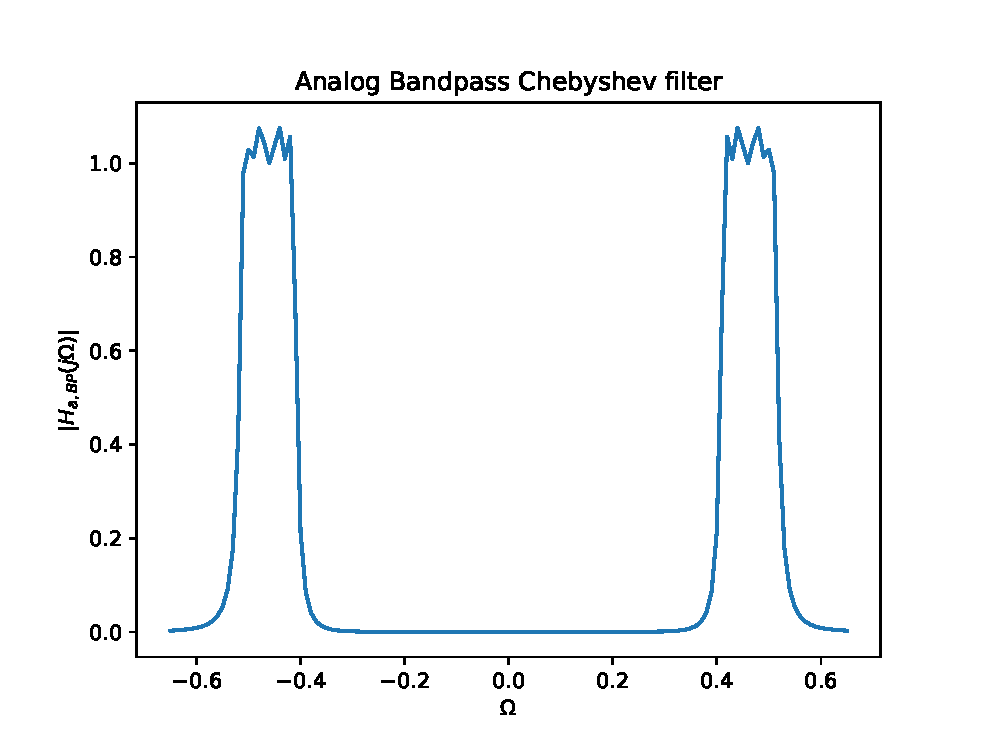
\includegraphics[width=0.30\columnwidth]{./figs_iir/ee18btech11034_Analog_IIR_Bandpass.eps}
\caption{Analog Bandpass IIR filter magnitude response}
\label{fig:Figure8}
\end{figure}
\end{frame}
\begin{frame}
\begin{figure}[!h]
%\centering
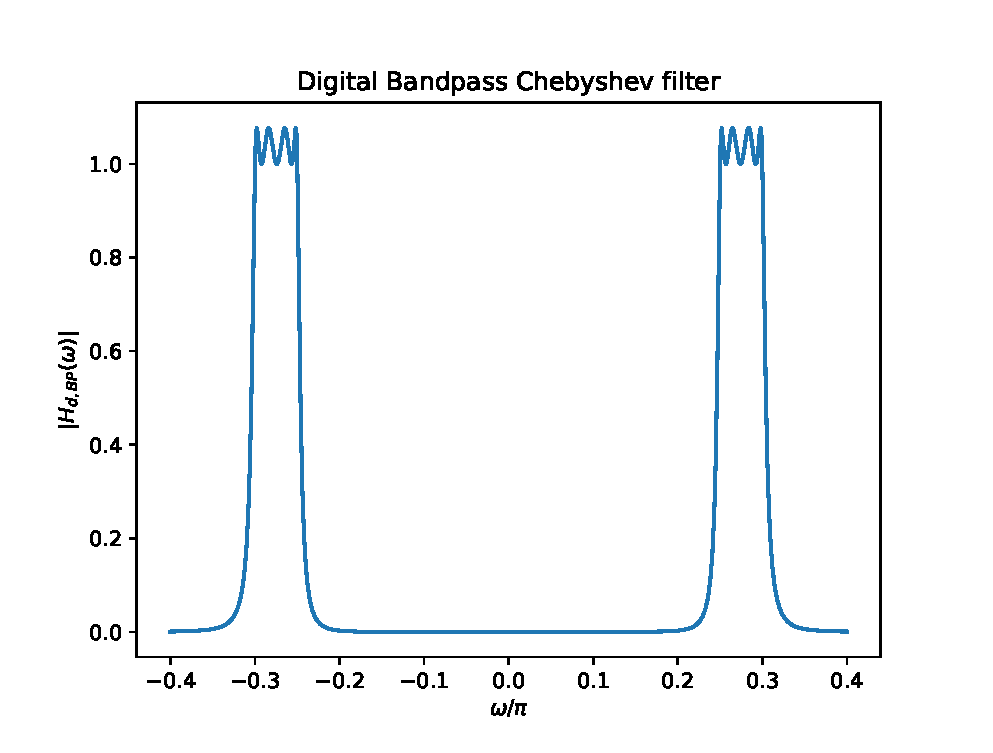
\includegraphics[width=0.75\columnwidth]{./figs_iir/ee18btech11034_Digital_IIR_Bandpass.eps}
\caption{Digital Bandpass IIR filter magnitude response vs Normalized Frequency}
\label{fig:Figure9}
\end{figure}
\end{frame}
\begin{frame}{FIR Filter Design}
The general impulse response $h_{lp}(n)$ for the desired lowpass FIR filter with cutoff frequency $\omega_{l}$ is given by 
\begin{align}
h_{l}(n) = \frac{\sin(n\omega_{l})}{n\pi} w(n)
\end{align}
where $w(n)$ is the Kaiser window obtained from the design specifications.
\\
We obtain the desired low pass filter impulse as 
\begin{eqnarray}
%\label{firlpfinal}
h_{lp}(n) &=& \frac{\sin(\frac{n\pi}{40})}{n\pi} \indent -100 \leq n \leq 100 \nonumber \\
&=& 0, \hspace{2cm} \mbox{otherwise}
\end{eqnarray}
The Kaiser window in the interval [-100,100] is chosen to be 1
\\
\end{frame}
\begin{frame}
The desired band pass filter impulse response is obtained as 
\begin{equation}
h_{bp}(n) = 2h_{lp}(n)cos(n\omega_c)
\end{equation}
\\
Thus now we obtain
\begin{eqnarray}
%\label{firbpfinal}
h_{bp}(n) &=& \frac{2\sin(\frac{n\pi}{40}) \cos(\frac{11n\pi}{40})}{n\pi} \indent -100 \leq n \leq 100 \nonumber \\
&=& 0, \hspace{4cm} \mbox{otherwise}
\end{eqnarray}
\\
Multiplication of $\cos(n\omega_{c})$ with sinc function in time domain gives convolution of rectangular window function centered around 0 with two delta functions at $\omega_{c}$ which finally gives two rectangular window functions centered around $\omega_{c}$ (genral bandpass FIR function).
\end{frame}
\begin{frame}{Plots of magnitude response of lowpass and bandpass FIR filters}
\begin{figure}[!h]
%\centering
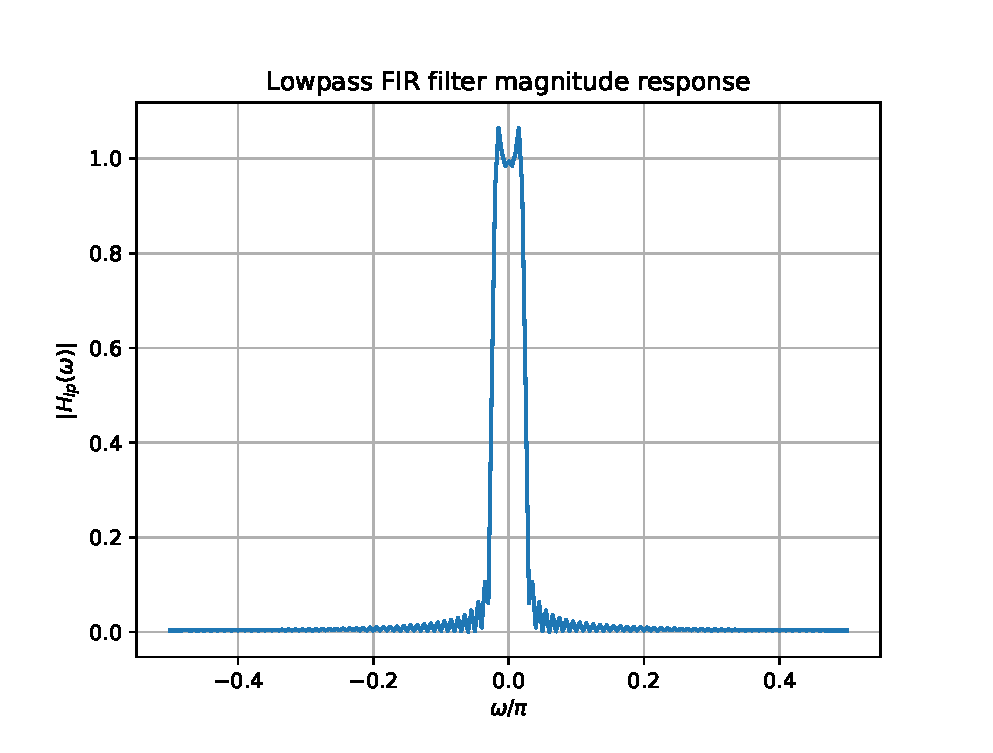
\includegraphics[width=0.30\columnwidth]{./figs_fir/ee18btech11034_FIR_Lowpass.eps}
\caption{Lowpass FIR filter magnitude response}
\label{fig:Figure10}
\end{figure}

\begin{figure}[!h]
%\centering
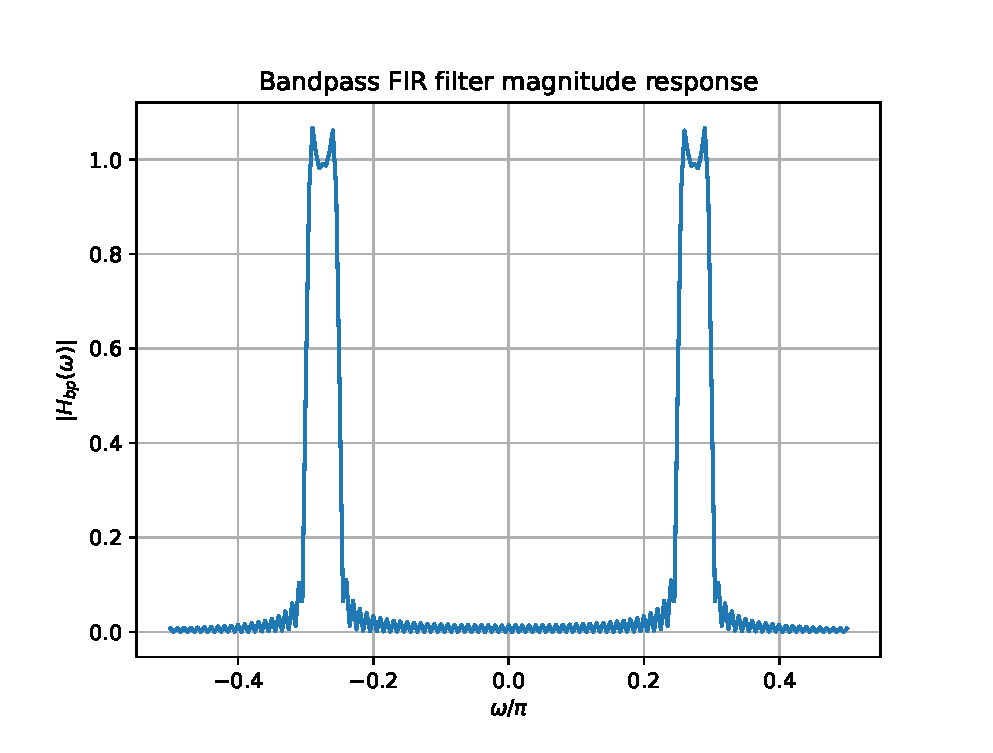
\includegraphics[width=0.30\columnwidth]{./figs_fir/ee18btech11034_FIR_Bandpass.eps}
\caption{Bandpass FIR filter magnitude response}
\label{fig:Figure11}
\end{figure}
\end{frame}
\end{document} 

